\documentclass{standalone}
\usepackage{preset}
\begin{document}
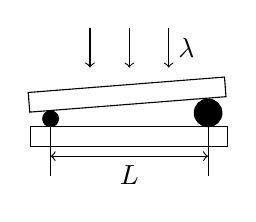
\begin{tikzpicture}[x=25mm,y=25mm]
	\draw(0,0)rectangle+(1,-.1);
	\draw[fill=black](.1,.04)circle(.04) (.9,.07)circle(.07);
	\draw[rotate=4.5](0,.074)rectangle+(1,.1);
	\draw(.1,.04)--(.1,-.25);
	\draw(.9,.07)--(.9,-.25);
	\draw[<->](.1,-.15)--node[below]{$L$}(.9,-.15);
	\draw[->](.3,.5)--+(0,-.2);
	\draw[->](.5,.5)--+(0,-.2);
	\draw[->](.7,.5)--node[right]{$\lambda$}+(0,-.2);
\end{tikzpicture}
\end{document}
